\chapter{Description des données}
\label{ch:description_donnees}

\section{Introduction}
Ce chapitre est consacré à la description approfondie du cycle de vie des données au sein de notre plateforme d’analyse de risques basée sur l’intelligence artificielle. La performance des algorithmes de détection de risques, de l’agent conversationnel (LangGraph + Mistral) et des simulations prédictives (Monte Carlo) dépend directement de la qualité, de la structure et de la fraîcheur des données extraites de l’écosystème Jira de NTT DATA Maroc. Nous détaillons d’abord les sources et les méthodes d’extraction des données, puis leur structure interne. Ensuite, nous présentons les analyses et visualisations clés qui alimentent le tableau de bord React. Enfin, nous décrivons le pipeline de normalisation et de préparation qui transforme les flux JSON bruts en signaux standardisés prêts à être consommés par les moteurs d’IA et de simulation.

\section{Source des données}
La source primaire et unique de notre plateforme est l’API REST de Jira (version 2), qui expose l’intégralité des données opérationnelles des projets logiciels suivis par NTT DATA Maroc. L’extraction est conçue pour être résiliente, asynchrone et respectueuse des limites de débit imposées par Jira.

\subsection{Authentification et endpoints utilisés}
L’accès à l’API est sécurisé par des sessions HTTP basées sur des jetons d’authentification (Basic Auth ou token personnel). Les principaux endpoints exploités sont :

\begin{figure}[H]
\centering
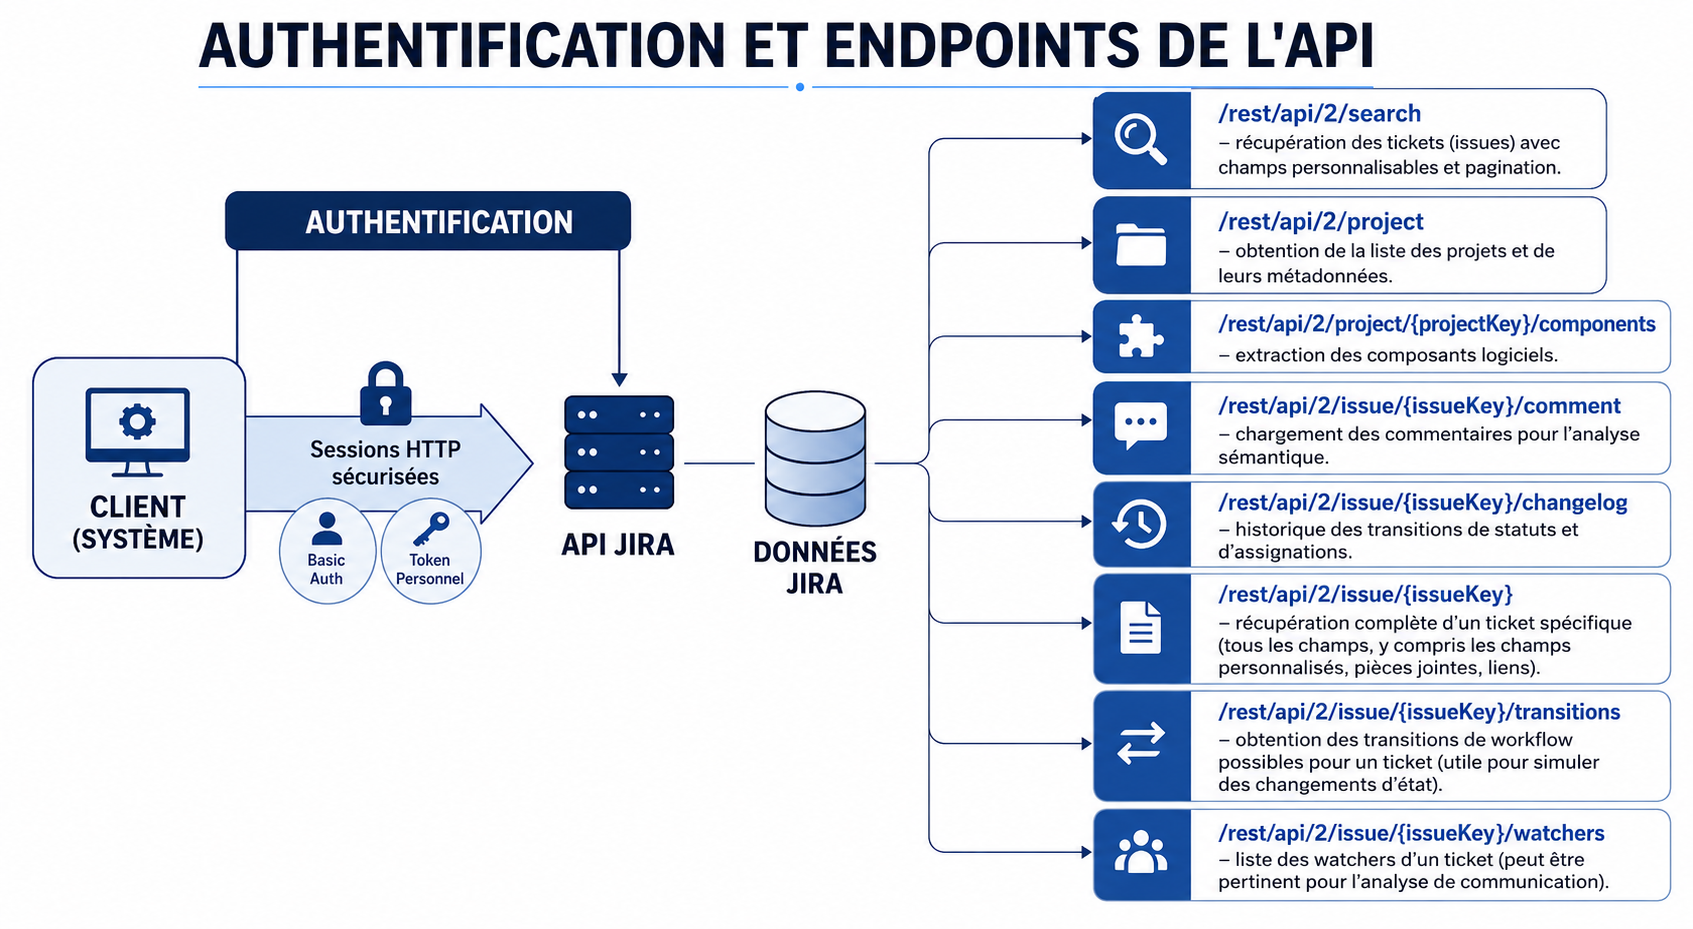
\includegraphics[width=0.9\linewidth]{assets/sourceD_authentification.png}
\caption{Schéma du mécanisme d’authentification à l’API Jira}
\label{fig:authentification}
\end{figure}    

\begin{itemize}
    \renewcommand{\labelitemi}{—}
    \item \texttt{/rest/api/2/search} : récupération des tickets (issues) avec champs personnalisables et pagination.
    \item \texttt{/rest/api/2/project} : obtention de la liste des projets et de leurs métadonnées.
    \item \texttt{/rest/api/2/project/\{projectKey\}/components} : extraction des composants logiciels.
    \item \texttt{/rest/api/2/issue/\{issueKey\}/comment} : chargement des commentaires pour l’analyse sémantique.
    \item \texttt{/rest/api/2/issue/\{issueKey\}/changelog} : historique des transitions de statuts et d’assignations.
    \item \texttt{/rest/api/2/issue/\{issueKey\}} : récupération complète d’un ticket spécifique (tous les champs, y compris les champs personnalisés, pièces jointes, liens).
    \item \texttt{/rest/api/2/issue/\{issueKey\}/transitions} : obtention des transitions de workflow possibles pour un ticket (utile pour simuler des changements d’état).
    \item \texttt{/rest/api/2/issue/\{issueKey\}/watchers} : liste des watchers d’un ticket (peut être pertinent pour l’analyse de communication).
\end{itemize}

\subsection{Requêtes JQL (Jira Query Language)}

Le \textbf{Jira Query Language (JQL)} est un langage de requête structuré propre à Jira Data Center, conçu pour interroger la base de données des tickets, projets, commentaires et historiques. Il permet de filtrer, trier et extraire uniquement les informations pertinentes selon des critères métiers précis (projet, dates, statuts, priorités, etc.). L’utilisation de JQL est essentielle pour limiter la charge sur l’API et ne conserver que les données nécessaires aux calculs de métriques et à l’entraînement de l’agent IA.

\paragraph{Bénéfices de l’utilisation de JQL dans notre plateforme}
\begin{itemize}
    \renewcommand{\labelitemi}{—}
    \item Réduction du volume de données transférées (seules les issues répondant aux critères temporels sont extraites).
    \item Amélioration des performances : les requêtes paginées sont exécutées plus rapidement grâce à des index optimisés par Jira.
    \item Flexibilité : adaptation dynamique des requêtes selon le contexte (analyse temps réel vs historique Monte Carlo).
    \item Respect des quotas de l’API (rate limiting) en limitant le nombre de tickets chargés.
\end{itemize}

\paragraph{Architecture de l’intégration des requêtes JQL dans l’application}

La figure \ref{fig:architecture_jql} illustre l’architecture d’intégration des requêtes JQL dans le backend FastAPI.
\begin{figure}[H]
\centering
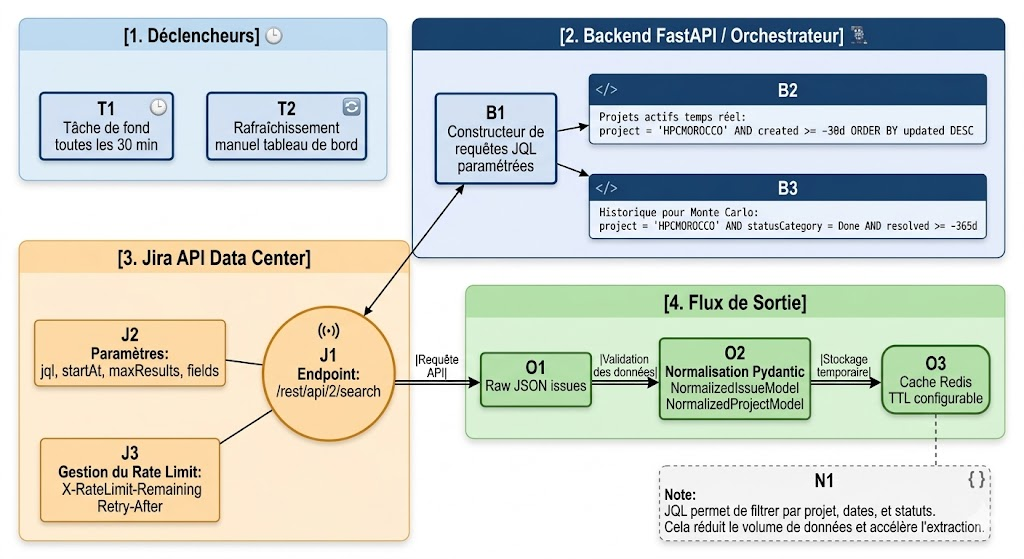
\includegraphics[width=0.9\linewidth]{assets/diagrams/arch_jql.jpg}
\caption{Intégration des requêtes JQL dans le backend FastAPI (architecture)}
\label{fig:architecture_jql}
\end{figure} 

La construction et l’exécution des requêtes JQL sont orchestrées par le backend FastAPI. Deux mécanismes de déclenchement sont mis en œuvre :
\begin{itemize}
    \renewcommand{\labelitemi}{—}
    \item \textbf{Tâche de fond} : toutes les 30 minutes, une routine asynchrone exécute une série de requêtes JQL prédéfinies (ex. historique des 365 derniers jours) pour maintenir le cache Redis à jour.
    \item \textbf{Requête à la demande} : lorsqu’un utilisateur rafraîchit le tableau de bord, le backend construit dynamiquement la requête JQL correspondant au projet sélectionné et aux filtres actifs (ex. “created >= -30d” pour les tickets récents).
\end{itemize}
Les requêtes sont paramétrées pour éviter les injections et garantissent la pagination automatique via \texttt{startAt} et \texttt{maxResults}. Les exemples suivants illustrent les deux cas d’usage principaux.

\paragraph{Exemples de requêtes utilisées}
Pour l’analyse temps réel des projets actifs :
\begin{verbatim}
project = "HPCMOROCCO" AND created >= -30d ORDER BY updated DESC
\end{verbatim}
Pour l’historique nécessaire aux simulations de Monte Carlo (vélocité) :
\begin{verbatim}
project = "HPCMOROCCO" AND statusCategory = Done AND resolved >= -365d
\end{verbatim}

Ces requêtes sont exécutées soit périodiquement par la tâche de fond, soit à la demande lors du rafraîchissement de l’interface.

\subsection{Gestion des limites de taux et optimisation}
L’API Jira impose des quotas stricts (ex. 100 requêtes par minute). Notre module \texttt{Fetch.py} implémente les mécanismes suivants :
\begin{itemize}
    \renewcommand{\labelitemi}{—}
    \item Détection des en‑têtes \texttt{X-RateLimit-Remaining} et \texttt{Retry-After}.
    \item Backoff exponentiel avec temporisation progressive en cas de réponse HTTP 429 (trop de requêtes) ou 503 (service indisponible).
    \item Parallélisation contrôlée par \texttt{ThreadPoolExecutor} pour les lots de tickets (batch de 200, soit 2 pages de 100), sans dépasser les limites.
\end{itemize}
La mise en cache des résultats est détaillée dans la section dédiée au stockage (cf. \ref{subsec:stockage_cache}).

\section{Description des données}
Les données brutes retournées par Jira sont au format JSON, riches mais hétérogènes. Le schéma standard de l’API Jira v2 structure l’information de la manière suivante : l’objet racine contient les métadonnées du ticket (clé, URL, etc.), et l’ensemble des champs métier est regroupé dans un objet \texttt{fields}. L’historique des transitions (\texttt{changelog}) est récupéré via un endpoint dédié et contient une liste d’entrées \texttt{histories}, chacune composée d’un timestamp et d’une liste d’items (\texttt{items}) décrivant les changements de champ.






\subsection{Champs des tickets (issues)}

La figure \ref{fig:jira_json_structure} présente un extrait d’un ticket Jira tel qu’il est retourné par l’API, mettant en évidence la structure imbriquée des champs.


\begin{figure}[H]
\centering
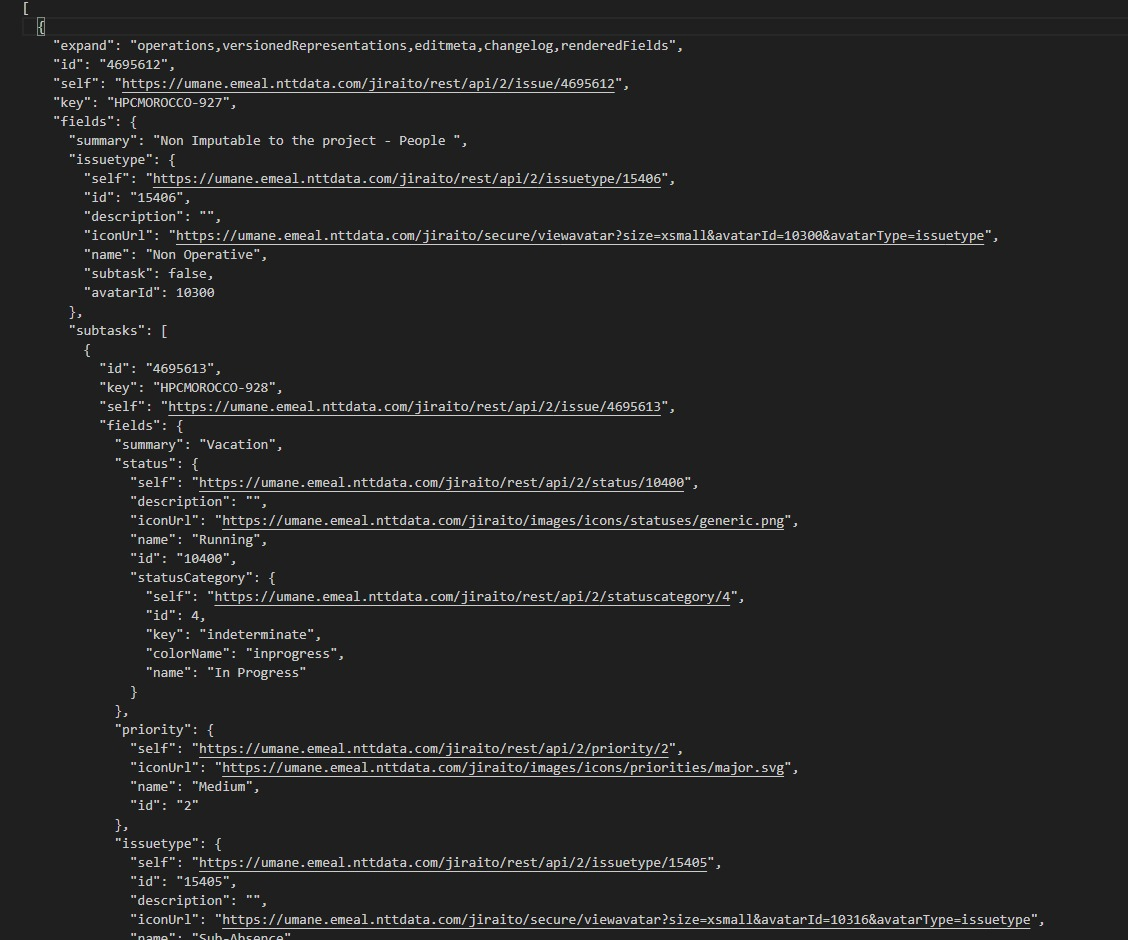
\includegraphics[width=0.9\linewidth]{assets/interfaces/json_screen.jpeg}
\caption{Extrait d’un ticket Jira au format JSON (structure imbriquée \texttt{fields}, \texttt{subtasks}, \texttt{statusCategory}, etc.)}
\label{fig:jira_json_structure}
\end{figure}
Chaque ticket est représenté par un objet contenant les champs suivants, sélectionnés pour leur pertinence dans les calculs métier et l’inférence IA :
\begin{itemize}
    \renewcommand{\labelitemi}{—}
    \item \textbf{Identité} : clé (ex. \texttt{HPCMOROCCO-123}), URL, résumé (\texttt{summary}), description (\texttt{description}).
    \item \textbf{Statut et typologie} : statut courant (\texttt{status}), catégorie de statut (\texttt{statusCategory} : \texttt{To Do}, \texttt{In Progress}, \texttt{Done}) permettant la normalisation des états pour le calcul du WIP ratio, type de ticket (\texttt{issuetype} : Bug, Tâche, Story, Épopée), priorité (\texttt{priority}).
    \item \textbf{Liens et dépendances} : champ \texttt{issuelinks} (bloque, est bloqué par, dépend de, etc.), essentiel pour la détection des risques en cascade et des tickets bloqués.
    \item \textbf{Dates} : création (\texttt{created}), dernière mise à jour (\texttt{updated}), échéance (\texttt{duedate}), résolution (\texttt{resolutiondate}).
    \item \textbf{Assignation} : assigné (\texttt{assignee}) avec son \texttt{accountId}, \texttt{displayName} et \texttt{avatarUrl} (exploités par le module Worker Insights pour identifier et visualiser les développeurs), rapporteur (\texttt{reporter}).
    \item \textbf{Estimations et charges} : estimation initiale (\texttt{timeoriginalestimate}), temps restant (\texttt{timeestimate}), temps passé (\texttt{timespent}), et Story Points (champ personnalisé \texttt{customfield\_10016}). Ce champ stocke la complexité estimée des tickets et est utilisé pour les calculs de vélocité et les simulations Monte Carlo.
    \item \textbf{Sprints} : champ personnalisé (ex. \texttt{customfield\_10020}) contenant les informations de sprint (nom, dates de début et de fin). Ce champ permet de regrouper les tickets par itération pour l’analyse de vélocité historique et le suivi de l’avancement agile.
    \item \textbf{Composants et versions} : liste des composants logiciels, versions d’affectation et de correction.
\end{itemize}

\subsection{Commentaires et historique}
L’analyse sémantique (risques cachés, blocages implicites) nécessite l’accès aux commentaires et aux changements d’état. Nous récupérons pour chaque ticket :
\begin{itemize}
    \renewcommand{\labelitemi}{—}
    \item \textbf{Commentaires} : auteur, date, contenu textuel.
    \item \textbf{Changelog} : chaque transition (\texttt{status}, \texttt{assignee}, \texttt{resolution}) avec ancienne valeur, nouvelle valeur et date de changement.
\end{itemize}
Ces données sont conservées sous forme de listes associées au ticket. Le \textit{changelog} est ensuite aplati pour extraire la date de dernière transition et calculer le temps passé dans chaque statut (cycle time), comme détaillé dans la section \ref{subsec:normalisation}.

\subsection{Métadonnées de projet}
Les informations générales sur les projets (clé, nom, catégorie, lead, type) sont stockées séparément pour enrichir les analyses contextuelles. Elles sont conservées dans le cache Redis et rafraîchies périodiquement.

\subsection{Volumétrie et pagination}
Un projet actif de taille moyenne chez NTT DATA peut contenir plusieurs milliers de tickets. Pour éviter les limites de pagination de l’API Jira (50 ou 100 résultats par appel), nous utilisons la pagination basée sur le champ \texttt{startAt} avec une taille de page fixée à 100 tickets. Les appels sont parallélisés par lots de 2 pages consécutives (soit 200 tickets par lot) afin d’accélérer l’extraction de l’historique complet (par exemple, sur une fenêtre de 365 jours) en moins de 30 secondes.

\section{Analyse et Visualisation des Données}
Notre plateforme ne se limite pas à un affichage brut ; elle transforme les données Jira en indicateurs d’aide à la décision (KPI), en alertes de risque et en prévisions. Les visualisations sont intégrées au tableau de bord React à l’aide de bibliothèques comme Recharts ou Plotly.

\subsection{Analyse prédictive par Monte Carlo}
\label{subsec:montecarlo_visu}
La simulation Monte Carlo est utilisée pour prévoir la date de fin du projet en fonction du backlog restant et de la vélocité historique. Le processus est le suivant :
\begin{enumerate}
    \item Extraction des tickets résolus sur les 365 derniers jours.
    \item Calcul de la vélocité hebdomadaire (nombre de tickets clôturés par semaine). On obtient une distribution empirique.
    \item Comptage du nombre de tickets actuellement ouverts (non résolus).
    \item Simulation de 10\,000 scénarios : chaque semaine, on tire aléatoirement une vélocité dans la distribution historique, on soustrait le backlog jusqu’à ce qu’il soit nul.
    \item On extrait les percentiles (p50, p75, p85, p95) des dates de fin obtenues.
\end{enumerate}
L’interface affiche une courbe de probabilité cumulée et un intervalle de confiance. Par exemple, pour le projet pilote \texttt{HPCMOROCCO}, la simulation indique qu’il y a \textbf{90\,\% de chances} que le projet soit terminé avant le 15 décembre, et \textbf{85\,\% de chances} avant le 10 décembre (intervalle p85). Les percentiles p50, p75, p85 et p95 sont également affichés sous forme de repères sur la courbe.

\subsection{Visualisation des métriques de santé projet}
Les métriques de santé projet (WIP ratio, stale ratio, overdue rate, coefficient de Gini) sont calculées en temps réel (leur définition et leur évaluation sont détaillées dans le chapitre 4). Elles sont affichées sous forme de cartes de valeur, de jauges colorées et de courbes d’évolution temporelle dans le tableau de bord principal. Ces indicateurs permettent aux chefs de projet de détecter instantanément les dérives et les goulots d’étranglement.

\subsection{Visualisation du module Worker Insights}
Le module Worker Insights présente une grille adaptative de cartes développeur. Chaque carte affiche le nom, le projet, le nombre de tickets assignés, terminés, en cours et bloqués, ainsi que des badges de charge (\texttt{OVERLOADED}, \texttt{BALANCED}, \texttt{UNDERUTILIZED}) et de performance (\texttt{ABOVE\_AVERAGE}, \texttt{AVERAGE}, \texttt{BELOW\_AVERAGE}). Un clic sur \textit{View AI Insight} ouvre un panneau latéral détaillant l’analyse complète générée par l’agent IA (résumé textuel, commentaires par ticket, évaluation de charge, recommandations). Les données sous‑jacentes sont préparées par une agrégation par assignee (cf. section \ref{subsec:worker_aggregation}).

\subsection{Explorateur Jira et supervision Grafana}
Par ailleurs, le tableau de bord intègre un explorateur Jira permettant de filtrer et visualiser les tickets par statut, priorité ou assigné. En complément, la stack de supervision (Grafana) offre des tableaux de bord dédiés à l’évolution temporelle des métriques et à l’état des alertes, comme décrit dans le chapitre 4.

\section{Préparation des données}
\label{subsec:preparation}
Avant toute analyse, les données brutes issues de Jira subissent un pipeline de normalisation et de transformation. Ce pipeline est implémenté dans les modules \texttt{Fetch.py}, \texttt{Normalisation.py} et \texttt{metrics.py}.

\begin{figure}[H]
\centering
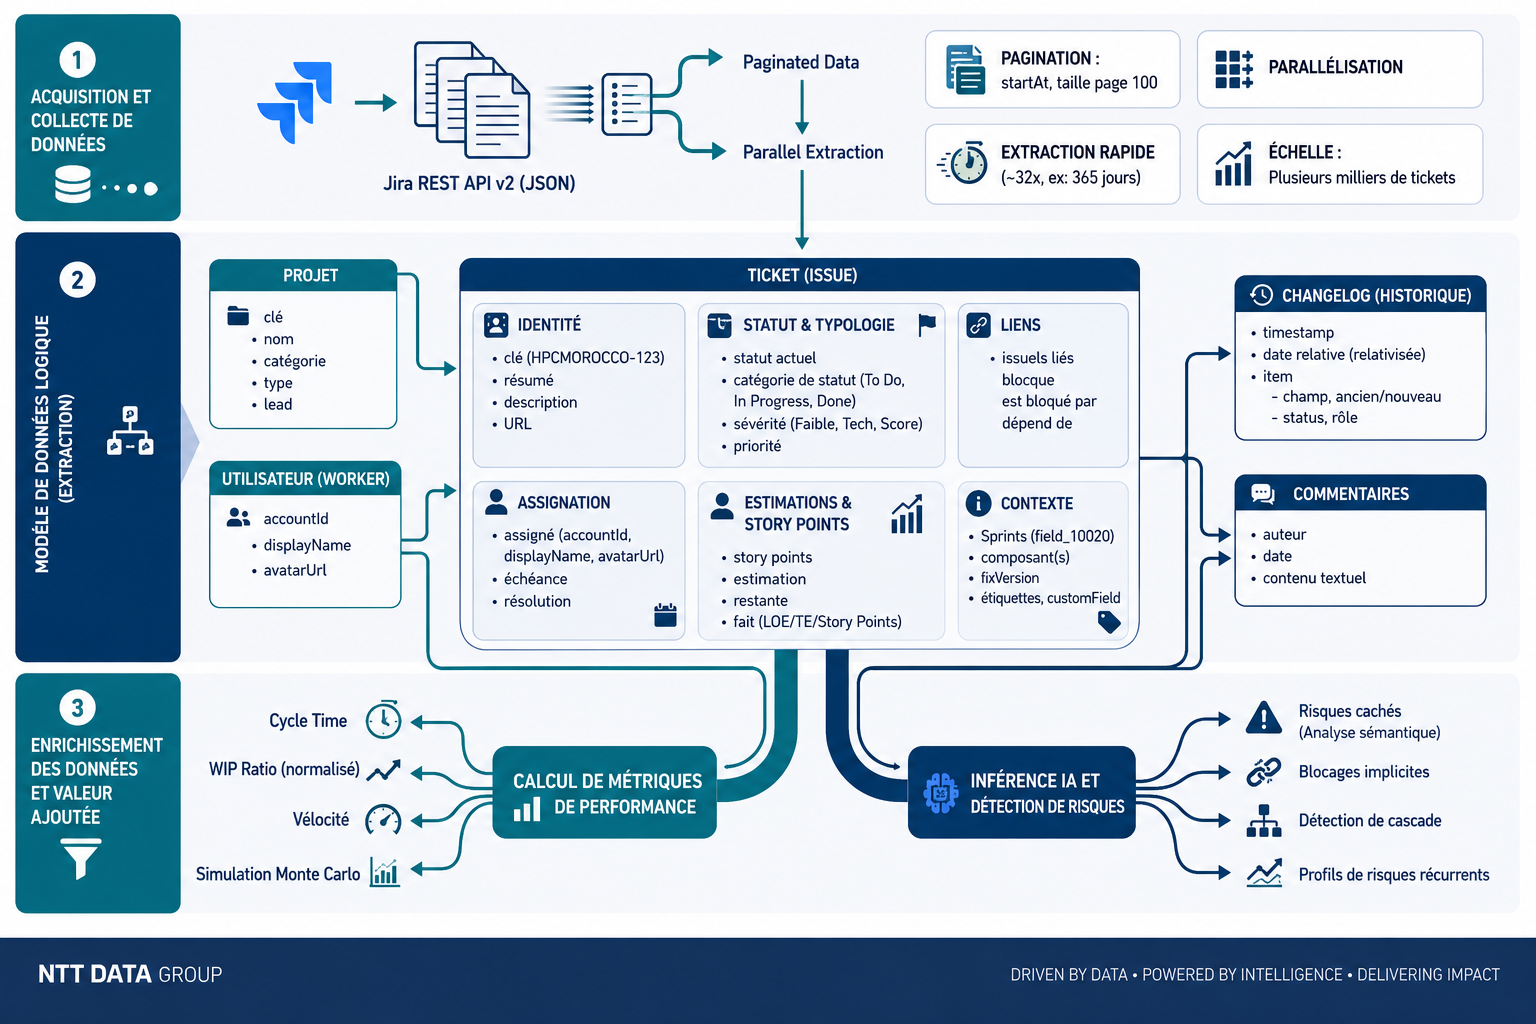
\includegraphics[width=0.9\linewidth]{assets/description_donnees.png}
\caption{Processus de traitement des données Jira et flux de métriques}
\label{fig:processus_donnees}
\end{figure}

Le processus global de traitement des données est illustré par la figure \ref{fig:processus_donnees}.

\subsection{Normalisation structurelle et aplatissement du changelog}
\label{subsec:normalisation}
Le JSON hétérogène retourné par l’API est passé dans des modèles Pydantic stricts (ex. \texttt{NormalizedIssueModel}) qui :
\begin{itemize}
    \renewcommand{\labelitemi}{—}
    \item Valident les types et la présence des champs obligatoires.
    \item Réorganisent l’information en quatre blocs : \texttt{identity}, \texttt{temporality}, \texttt{semantics}, \texttt{actors}.
    \item Convertissent les chaînes ISO en objets \texttt{datetime} (fuseau UTC) pour faciliter les calculs temporels.
    \item Aplatissent le \texttt{changelog} pour extraire la date de dernière transition et calculer le temps passé dans chaque statut (cycle time) – ce qui permet de déterminer \texttt{days\_since\_update} pour les tickets.
\end{itemize}
La normalisation élimine les variations inutiles (ex. champs \texttt{fields} imbriqués) et produit un objet Python homogène.

\subsection{Standardisation sémantique}
Les statuts Jira étant libres et personnalisables par chaque projet, nous appliquons une fonction de mappage (\texttt{jira\_canonical\_status}) qui traduit les noms bruts (ex. “En Cours”, “In Progress”, “Open”) vers quatre catégories canoniques :
\begin{itemize}
    \renewcommand{\labelitemi}{—}
    \item \texttt{todo} : tout statut initial ou ouvert non commencé.
    \item \texttt{in\_progress} : travail engagé.
    \item \texttt{done} : statuts de résolution (Fermé, Résolu, Livré).
    \item \texttt{unknown} : statut non reconnu (pour debug).
\end{itemize}
Cette standardisation permet de calculer le WIP ratio indépendamment des conventions de nommage.

\subsection{Agrégation pour le module Worker Insights}
\label{subsec:worker_aggregation}
Le module Worker Insights nécessite une préparation spécifique des données par développeur. La fonction \texttt{\_build\_worker\_snapshots()} regroupe les tickets par \texttt{assignee} et calcule pour chaque développeur les métriques suivantes : total de tickets assignés, tâches terminées, en cours, bloquées, taux de retard et temps de cycle moyen. Ces indicateurs sont complétés par les moyennes d’équipe (\texttt{avg\_completed}, \texttt{avg\_wip}, \texttt{avg\_assigned}) servant de référentiel de comparaison pour l’agent IA.

\subsection{Ingénierie des caractéristiques et préparation du contexte LLM}
Pour la simulation Monte Carlo, nous transformons l’historique des résolutions en un vecteur de comptages hebdomadaires (modèle « sac de billes ») afin d’optimiser les tirages aléatoires vectorisés via NumPy. Par ailleurs, pour l’agent IA, nous assemblons un prompt système structuré qui injecte les métriques calculées, les résultats du moteur de règles et les tickets actifs. La gestion de la fenêtre de contexte (limite de tokens) est assurée par la bibliothèque \texttt{tiktoken}, garantissant que la requête adressée à Mistral respecte les capacités du modèle.

\subsection{Stockage et mise en cache}
\label{subsec:stockage_cache}
Pour éviter des appels répétitifs à l’API et garantir la réactivité, une stratégie de cache multi‑niveaux est mise en œuvre :
\begin{itemize}
    \renewcommand{\labelitemi}{—}
    \item Les tickets normalisés sont stockés dans Redis avec une clé du type \texttt{project:HPCMOROCCO:issues} et un TTL de 15 minutes.
    \item Les résultats de la simulation Monte Carlo sont conservés pendant 24 heures (car l’historique varie peu à court terme).
    \item Les snapshots du module Worker Insights sont mis en cache avec un TTL de 15 minutes.
    \item En cas d’indisponibilité de Redis, le système bascule sur des fichiers JSON locaux (cache de secours) pour ne pas interrompre le service.
\end{itemize}

\section{Conclusion}
Ce chapitre a exposé l’intégralité du cycle de vie des données au sein de notre plateforme : extraction depuis l’API REST de Jira via des requêtes JQL optimisées, normalisation rigoureuse via des modèles Pydantic (incluant l’aplatissement du changelog), calcul de métriques de santé projet, simulation prédictive par Monte Carlo, agrégation pour le module Worker Insights, préparation du contexte pour le LLM, et visualisation dans un tableau de bord React ainsi que dans Grafana. La mise en cache intelligente (Redis) et les mécanismes de résilience garantissent des performances élevées tout en respectant les quotas de l’API. Ces données préparées et enrichies servent directement de combustible à l’agent IA conversationnel (LangGraph + Mistral) et aux algorithmes de détection de risques, dont l’implémentation est détaillée dans le chapitre suivant.